%%%%%%%%%%%%%%%%%%%%%%%%%%%%%%%%%%%%%%%%%%%%%%%%%%%%%%%%%%%%%%%%%%%%%%
% Overleaf (WriteLaTeX) Example: Molecular Chemistry Presentation
%
% Source: http://www.overleaf.com
%
% In these slides we show how Overleaf can be used with standard 
% chemistry packages to easily create professional presentations.
% 
% Feel free to distribute this example, but please keep the referral
% to overleaf.com
% 
%%%%%%%%%%%%%%%%%%%%%%%%%%%%%%%%%%%%%%%%%%%%%%%%%%%%%%%%%%%%%%%%%%%%%%

\documentclass{beamer}

\mode<presentation>
{
  \usetheme{Madrid}       % or try default, Darmstadt, Warsaw, ...
  \usecolortheme{default} % or try albatross, beaver, crane, ...
  \usefonttheme{default}    % or try default, structurebold, ...
  \setbeamertemplate{navigation symbols}{}
  \setbeamertemplate{caption}[numbered]
} 

\usepackage[english]{babel}
\usepackage[utf8x]{inputenc}
\usepackage{chemfig}
\usepackage[version=3]{mhchem}

\usepackage{hyperref}
  \hypersetup{colorlinks=true}
  \hypersetup{urlcolor=blue}
  \hypersetup{linkcolor = .}
\usepackage{xcolor}
\usepackage{siunitx}
  \sisetup{separate-uncertainty = true}
\usepackage{physics}
\usepackage[font=small,labelfont=bf]{caption}
\usepackage{subcaption}
\usepackage[en-GB]{datetime2}
\usepackage{feynmp}
\DeclareGraphicsRule{*}{mps}{*}{}

% Here's where the presentation starts, with the info for the title slide
\title[Graduate Symposium]{Anomalous Cherenkov rings in the DELPHI detector:\\A search for tachyons}
\author{Martin Tat}
\institute{University of Oxford}
\date{15th February 2021}

\titlegraphic{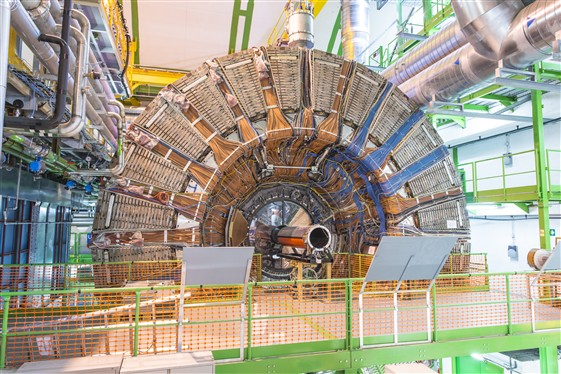
\includegraphics[width = 5cm, height = 3cm]{DELPHI_CERN.jpg}\hspace{1cm}~%
              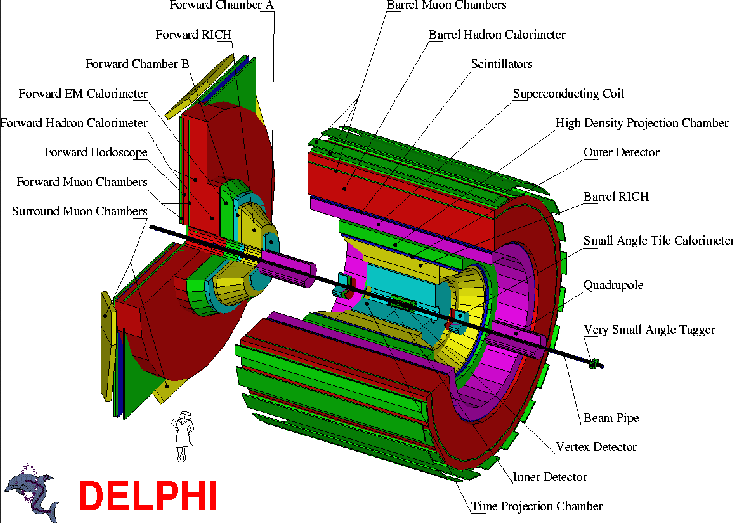
\includegraphics[width = 5cm, height = 3cm]{delphi.png}}

\begin{document}

\begin{frame}
  \titlepage
\end{frame}

% These three lines create an automatically generated table of contents.
\begin{frame}{Outline}
  \tableofcontents
\end{frame}

\section{Introduction}
\begin{frame}{Introduction}
  \begin{itemize}
    \item{Physical interpretation of the anomalous Cherenkov rings observed with the DELPHI detector}
    \begin{itemize}
      \item{\href{https://arxiv.org/abs/2001.08576v1}{arXiv:2001.08576}}
      \item{Retired HEP scientists?}
      \item{Independent of DELPHI Collaboration}
    \end{itemize}
    \item{Interpret large Cherenkov rings as tachyons}
    \item{Measure mass parameter}
  \end{itemize}
\end{frame}

\section{DELPHI and RICH}
\begin{frame}{DELPHI and RICH}
  \begin{itemize}
    \item{DELPHI: Detector with Lepton, Photon and Hadron Identification}
    \begin{itemize}
      \item{One of four main detectors at LEP}
      \item{Operated from $1989$ to $2000$}
      \item{Used RICH for PID}
    \end{itemize}
    \item{DELPHI Barrel RICH:}
    \begin{itemize}
      \item{Cherenkov angle: $\cos(\theta) = \frac{1}{n\beta}$}
      \item{$C_6F_{14}$ liquid radiator ($n = 1.273 \implies \theta_\text{max} = \SI{667}{\milli\radian}$)}
      \item{$C_5F_{12}$ gaseous radiator($n = 1.00194 \implies \theta_\text{max} = \SI{62}{\milli\radian}$)}
    \end{itemize}
  \end{itemize}
\end{frame}

\begin{frame}{DELPHI and RICH}
  \begin{figure}
    \centering
    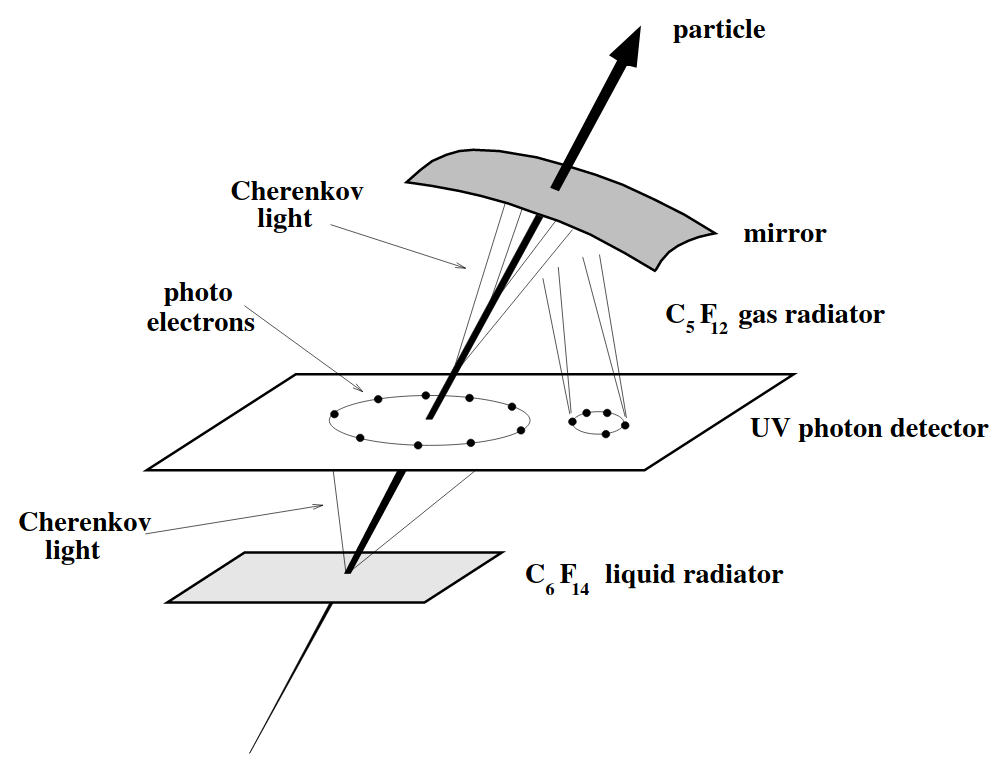
\includegraphics[width = 0.50\textwidth]{Cherenkov.png}
    \caption{Principles of the DELPHI RICH detector}
  \end{figure}
  \begin{itemize}
    \item{DELPHI strategy: Fit rings with five mass hypothesis ($e$, $\mu$, $\pi$, $K$, $p$) to obtain Cherenkov angle}
    \item{This paper: Fit each photon direction individually}
  \end{itemize}
\end{frame}

\section{Tachyon particles}
\begin{frame}{Tachyon particles}
  \begin{itemize}
    \item{Particles moving at $v > c$}
    \item{$E^2 - p^2 = -\mu^2$}
    \item{$\mu$: Mass parameter}
    \item{$\mu = p\sqrt{1 - n^2\cos^2(\theta)}$}
  \end{itemize}
\end{frame}

\section{Event topologies and candidate selection}
\begin{frame}{Event topologies and candidate selection}
  \begin{itemize}
    \item{Topology $1$: $e^+e^-\to\gamma t^+t^-$}
    \begin{itemize}
      \item{High energy photon back-to-back with tachyons}
      \item{Signature:}
      \begin{itemize}
        \item{One neutral and one charged jet}
        \item{Use $\dd{E}/\dd{x}$ to distinguish from single tracks}
        \item{Charged jet should shower in EM calorimeter}
      \end{itemize}
    \end{itemize}
  \end{itemize}
  \begin{figure}
    \centering
    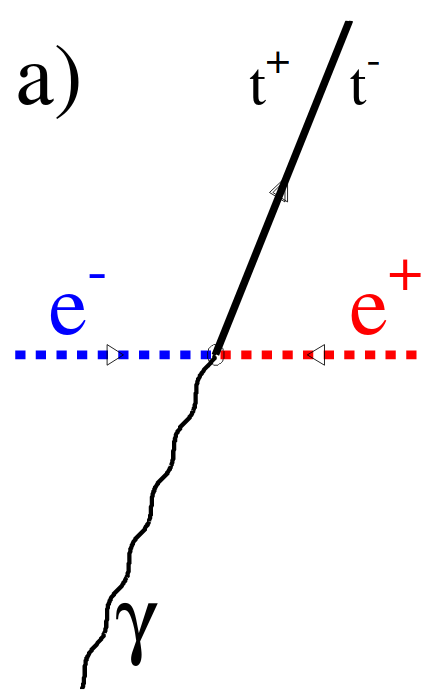
\includegraphics[width = 0.2\textwidth]{TopologyA.png}
  \end{figure}
\end{frame}

\begin{frame}{Event topologies and candidate selection}
  \begin{figure}
    \centering
    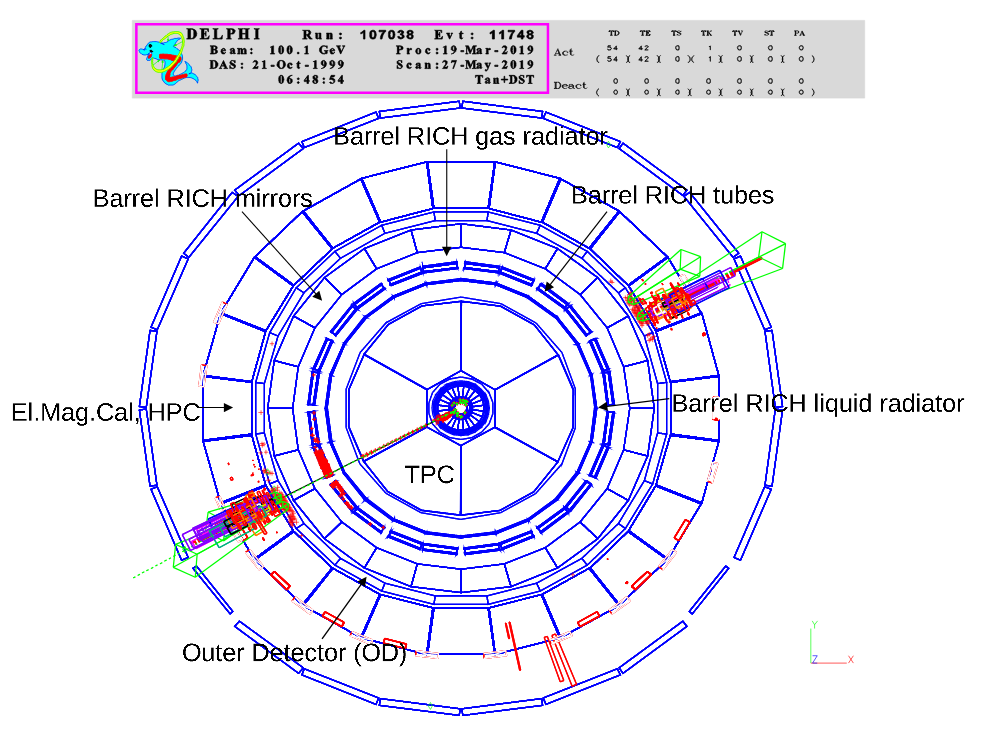
\includegraphics[width = 0.6\textwidth]{Topology1.png}
    \caption{$e^+e^-\to \gamma t^+t^-$ event}
  \end{figure}
\end{frame}

\begin{frame}{Event topologies and candidate selection}
  \begin{itemize}
    \item{Topology $2a$: $e^+e^-\to t^+t^-$}
    \item{Topology $2b$: $e^+e^-\to e^+e^-t^+t^-$}
    \begin{itemize}
      \item{Tachyon pair production}
      \item{Signature:}
      \begin{itemize}
        \item{Both tracks should have showers in EM calorimeter}
        \item{Tracks in opposite directions and opposite charge}
      \end{itemize}
    \end{itemize}
  \end{itemize}
  \begin{figure}
    \centering
    \begin{subfigure}{0.5\textwidth}
      \centering
      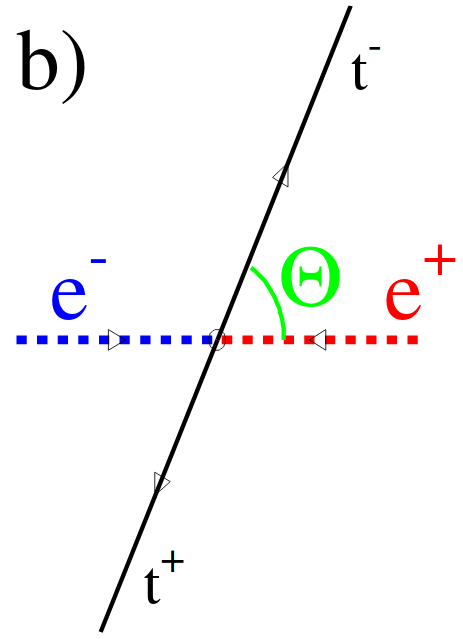
\includegraphics[width = 0.4\textwidth]{TopologyB.png}
    \end{subfigure}%
    \begin{subfigure}{0.5\textwidth}
      \centering
      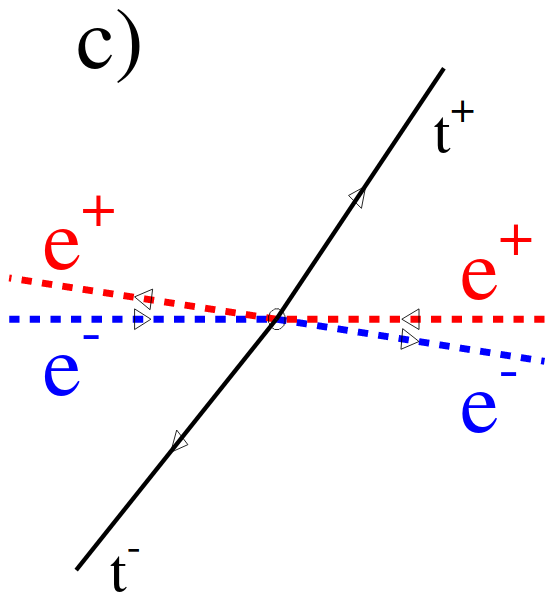
\includegraphics[width = 0.4\textwidth]{TopologyC.png}
    \end{subfigure}
  \end{figure}
\end{frame}

\begin{frame}{Event topologies and candidate selection}
  \begin{figure}
    \centering
    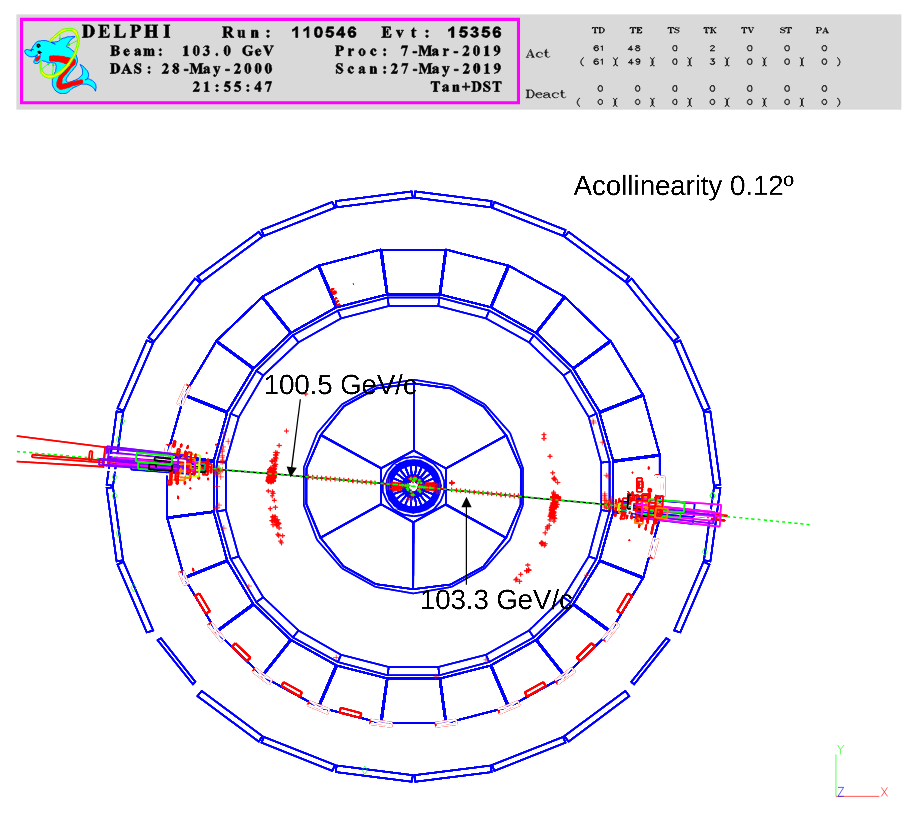
\includegraphics[width = 0.6\textwidth]{Topology2.png}
    \caption{$e^+e^-\to t^+t^-$ event}
  \end{figure}
\end{frame}

\begin{frame}{Event topologies and candidate selection}
  \begin{itemize}
    \item{Topology $3$: $eX\to eX't^+t^-$}
    \begin{itemize}
      \item{$e^\pm$ interaction with matter to produce tachyons}
      \item{Signature:}
      \begin{itemize}
        \item{Two jets, one with a single track, one with $3$ charged tracks}
        \item{All tracks should shower in EM calorimeter}
        \item{Some tracks with non-zero impact parameters in the three-particle jet}
      \end{itemize}
    \end{itemize}
  \end{itemize}
  \begin{figure}
    \centering
    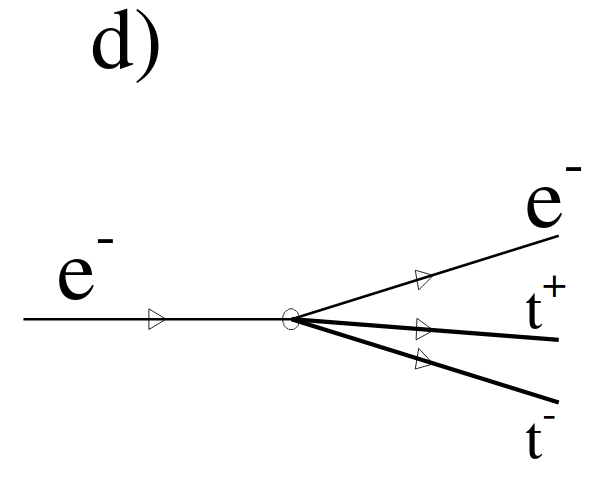
\includegraphics[width = 0.3\textwidth]{TopologyD.png}
  \end{figure}%
\end{frame}

\begin{frame}{Event topologies and candidate selection}
  \begin{figure}
    \centering
    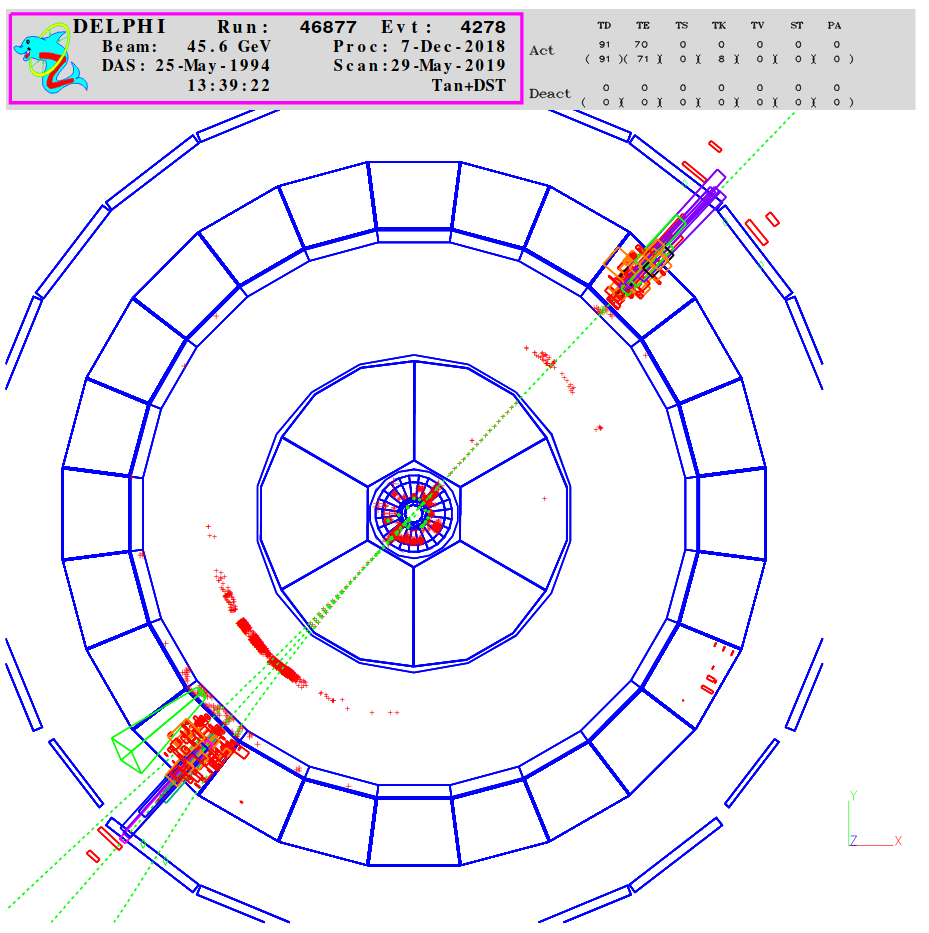
\includegraphics[width = 0.6\textwidth]{Topology3.png}
    \caption{$eX\to eX't^+t^-$ event}
  \end{figure}
\end{frame}

\begin{frame}{Event topologies and candidate selection}
  \begin{itemize}
    \item{Other general selection criteria: No hadrons, no muons, good track quality, etc...}
    \item{Result after selection:}
    \begin{itemize}
      \item{$53$ event with at least one anomalous Cherenkov ring}
      \item{$29$ candidates had two anomalous rings per track}
    \end{itemize}
  \end{itemize}
\end{frame}

\section{Analysis results}
\subsection{Correlation between RICH detectors}
\begin{frame}{Correlation between RICH detectors}
  \begin{itemize}
    \item{From Cherenkov angle formula:}
    \begin{itemize}
      \item{$n_1\cos(\theta_1) = \frac{1}{\beta} = n_2\cos(\theta_2)$}
      \item{Can plot this as a line in the $\theta_1$ vs $\theta_2$ plane}
    \end{itemize}
    \item{Or plot the predicted speeds $\beta_1$ and $\beta_2$}
  \end{itemize}
\end{frame}

\begin{frame}{Correlation between RICH detectors}
  \begin{figure}
    \centering
    \begin{subfigure}{0.5\textwidth}
      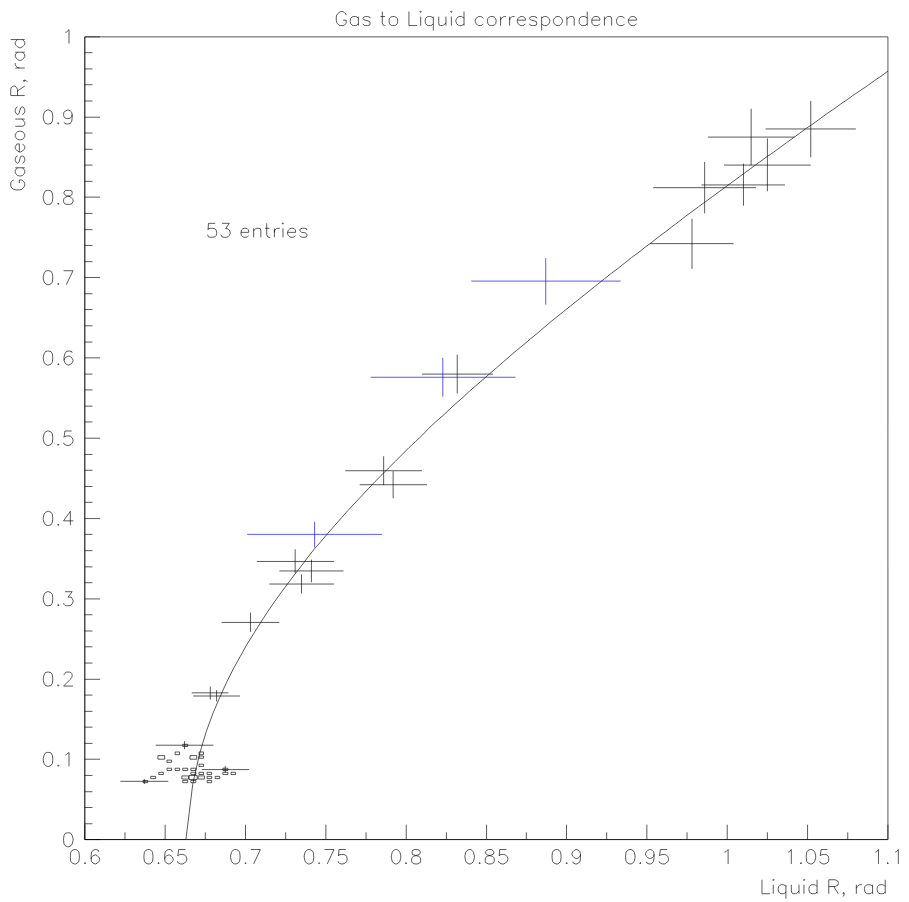
\includegraphics[width = 1\textwidth]{AngleCorrelation.png}
      \caption{Gas to liquid angle correlation}
    \end{subfigure}%
    \begin{subfigure}{0.5\textwidth}
      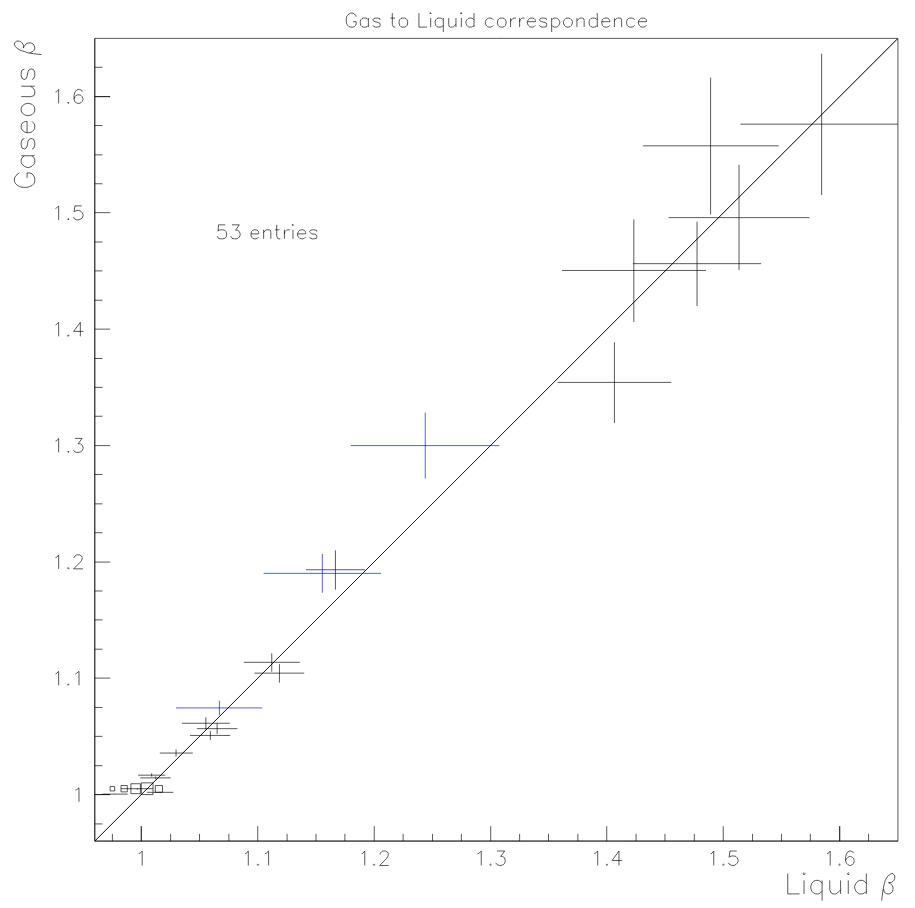
\includegraphics[width = 1\textwidth]{SpeedCorrelation.png}
      \caption{Gas to liquid speed correlation}
    \end{subfigure}
  \end{figure}
\end{frame}

\subsection{Tachyon mass parameters}
\begin{frame}{Tachyon mass parameters}
  \begin{itemize}
    \item{Calculate the mass parameters $\mu$ from Cherenkov angles}
    \item{Find correlation between Cherenkov radiators}
    \item{Found excess events at $\mu = \SI{0.28}{\giga\eV}$ and $\mu = \SI{5}{\giga\eV}$}
  \end{itemize}
  \begin{equation*}
    \mu = p\sqrt{1 - n^2\cos^2(\theta)}
  \end{equation*}
\end{frame}

\begin{frame}{Tachyon mass parameters}
  \begin{figure}
    \centering
    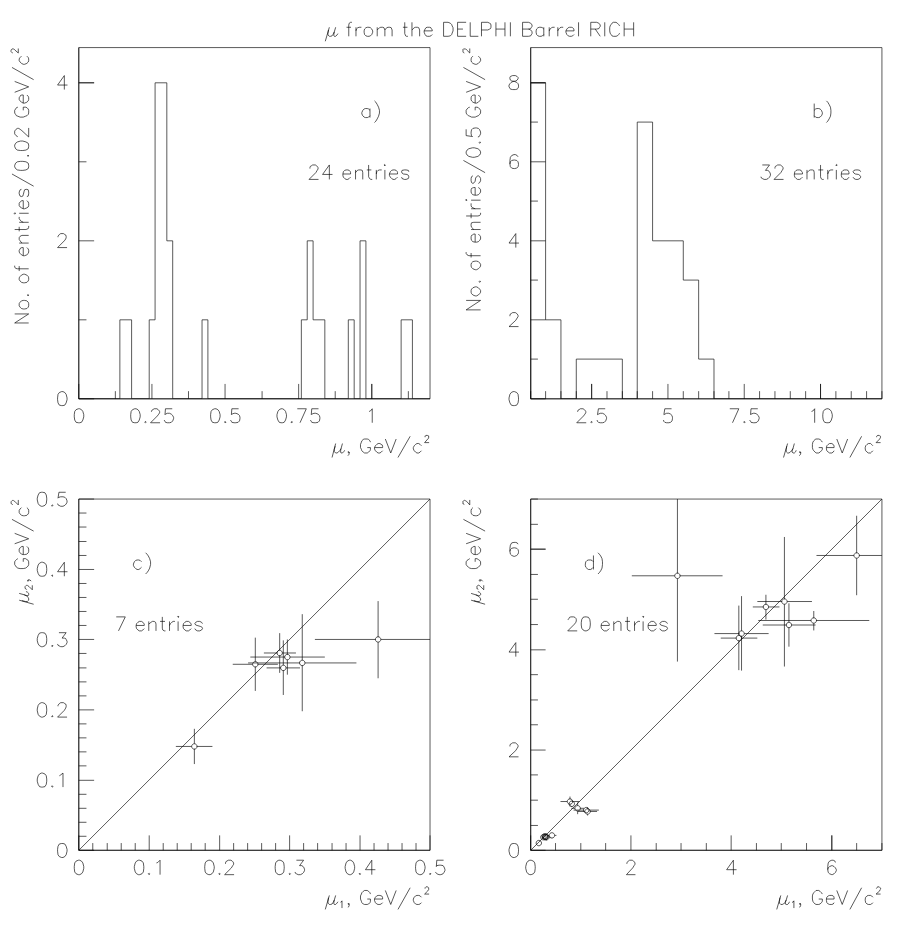
\includegraphics[width = 0.6\textwidth]{MassParameters.png}
    \caption{Tachyon mass parameters $\mu$}
  \end{figure}
\end{frame}

\subsection{Kinematic fit}
\begin{frame}{Kinematic fit}
  \begin{itemize}
    \item{Do an over-constrained kinematic fit}
    \item{$\mu$ is unknown}
    \item{Constraints:}
    \begin{itemize}
      \item{Energy-momentum conservation}
      \item{$\mu = p\sqrt{1 - n^2\cos^2(\theta)}$}
    \end{itemize}
  \end{itemize}
\end{frame}

\begin{frame}{Kinematic fit}
  \begin{figure}
    \centering
    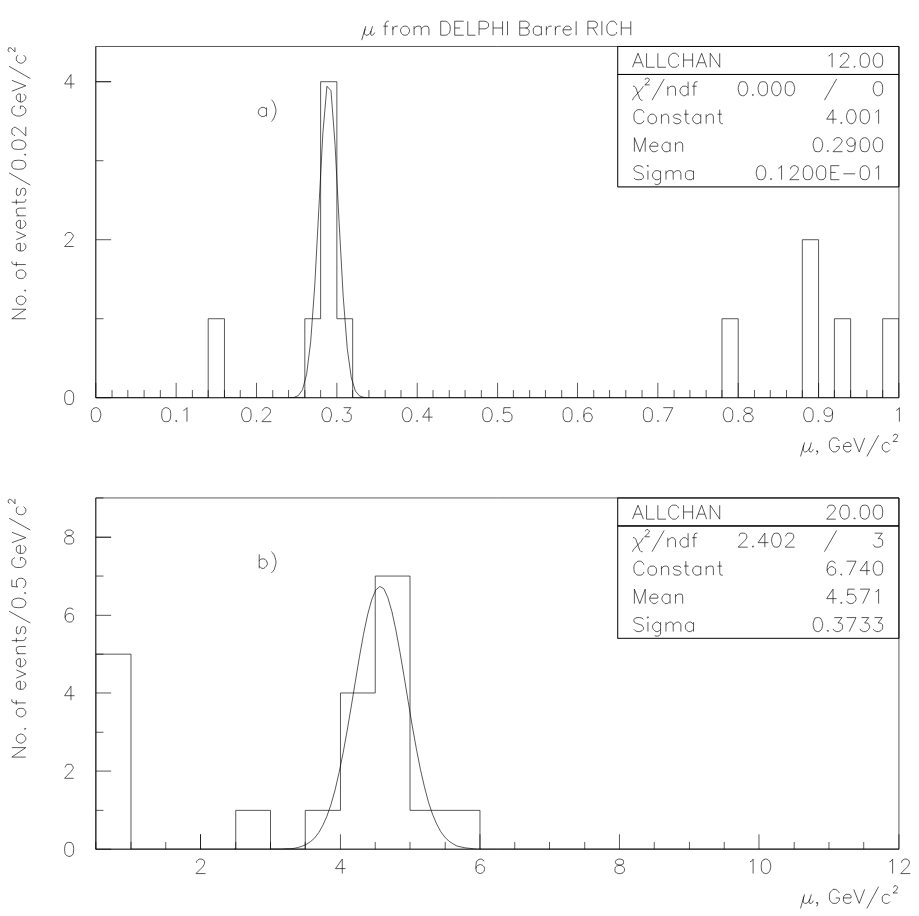
\includegraphics[width = 0.6\textwidth]{ConstrainedMassParameters.png}
    \caption{Tachyon mass parameters $\mu$ after kinematic fit}
  \end{figure}
\end{frame}

\section{Conclusion}
\begin{frame}{Conclusion}
  \begin{itemize}
    \item{Anomalous Cherenkov rings at DELPHI have been interpreted as tachyon signals}
    \item{Strong correlations between the gaseous and liquid RICH radiators were found}
    \item{Tachyon mass parameters show an excess at $\SI{0.29(1)}{\giga\eV}$ and $\SI{4.6(2)}{\giga\eV}$}
    \item{Further experiments are needed to confirm or refute these findings}
    \begin{itemize}
      \item{$\gamma\gamma$ interactions (topology $2b$) at ALICE could study this with their RICH, with a $Z^2$ enhancement in cross section}
      \item{LHCb, with high RICH Cherenkov angle resolution, could use low multiplicity events}
    \end{itemize}
  \end{itemize}
\end{frame}

\end{document}